\documentclass[main.tex]{subfiles}
\begin{document}

\begin{itemize}
    \item Flask replaced eel.
    \item Explain the frontend and backend, and how PyMongo is used for a
        database.
    \item Explain how to and from json methods were implemented in every QWAK
        class and why this is required.

\end{itemize}

In order to access the GUI, the user must clone the \texttt{GitHub} as
mentioned above, navigate to the \texttt{core} folder and run:
\begin{lstlisting}[style=commands]
$   python gui-main 
\end{lstlisting}

executing the script responsible for calling \texttt{Eel} which will open a
browser window directly to the home page. Here, we create \texttt{QWAK} objects
to be manipulated by the GUI, and we define new functions that call the desired
\texttt{QWAK} methods. These functions are necessary because \texttt{Eel}
requires us to \textit{expose} a function in order for it to be called by
JavaScript.\par 

There are two available options for simulation. The user can either perform a
continuous-time quantum walk for a single instance of time or define an
interval of time for a dynamic evolution of the CTQW. The static page in figure
\ref{fig:guiStaticPage} offers a graph-making tool created with the JavaScript
\texttt{Cytoscape} package. There are two ways of creating graphs:
\begin{enumerate}
    \item Through pre-defined \texttt{NetworkX} graphs that require inputting
        graph size and generator name. This will be fed through \texttt{Eel}
        and evaluated by Python. The appropriate \texttt{NetworkX} function is
        called, and the necessary data for \texttt{Cytoscape} to display the
        correct number of nodes and edges is later sent to JavaScript. However,
        the original graph layout is not preserved due to package limitations. 

    \item By navigating to the \textit{Custom Graph} in case the desired graph
        is not readily available in \texttt{NetworkX}. The user can add any
        number of nodes with a button, then turn on the drawing mode to connect
        said nodes. JavaScript will then calculate the adjacency matrix
        directly so that the quantum walk objects can be properly created. This
        method has the advantage of preserving graph layout.
\end{enumerate}
In the future, we plan to extend this tool to allow for the introduction of
weights so that directed and oriented quantum walks can be performed.\par

\begin{figure}[!h]
  \centering
  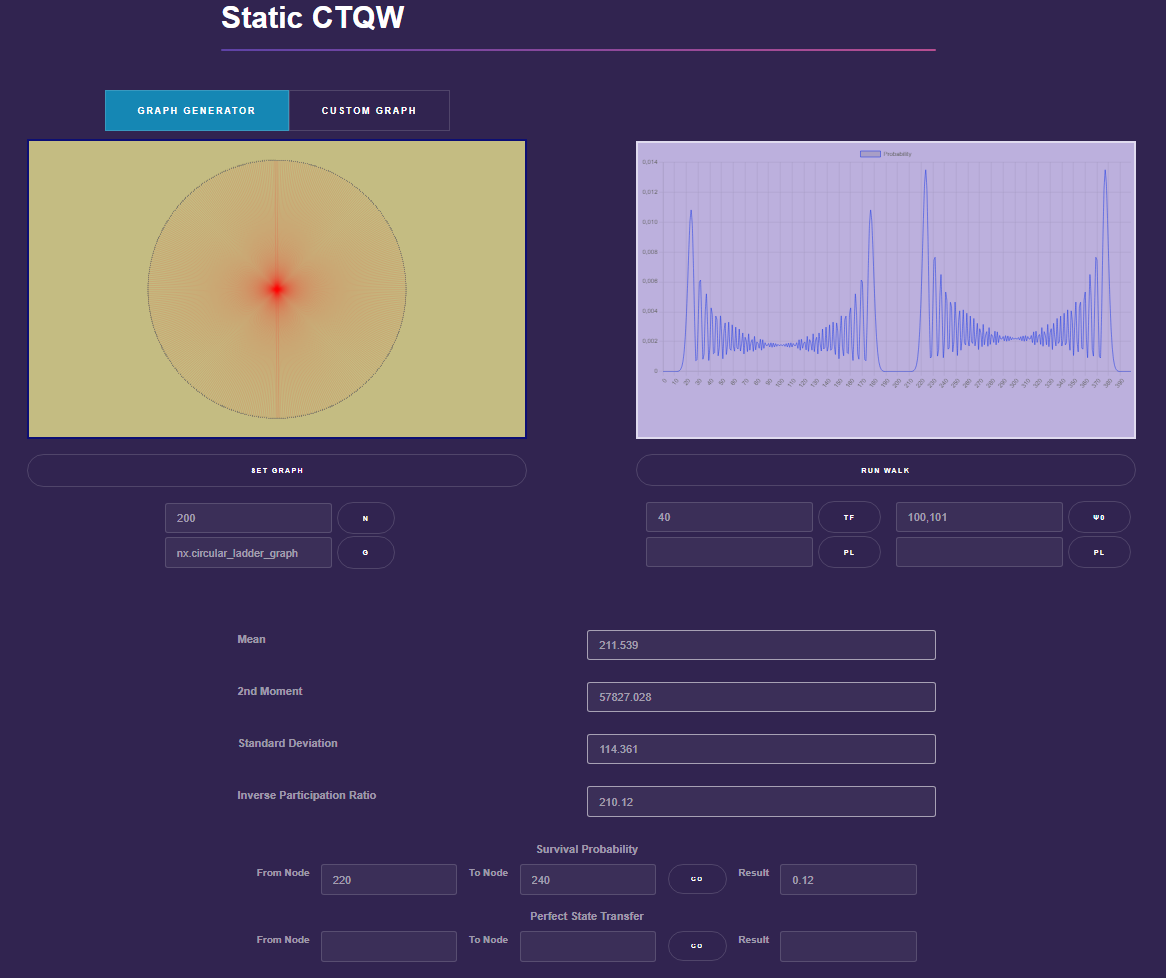
\includegraphics[scale=0.4]{img/QWAK/qwakGuiStaticQW.png}
  \caption{Graphical interface page of the static continuous-time quantum walk evolution.}
  \label{fig:guiStaticPage}
\end{figure}

To the right of the graph tool, we use \texttt{ChartJS} package to plot the
probability distributions. This is where the \texttt{buildWalk} method will be
called, and the user is required to specify the time and initial
condition. Currently, only the uniform superposition state can be created,
which will be expanded to allow custom states. After entering the desired
inputs, the user can press the \textit{Run Walk} button, signaling Python to
perform the evolution and return the probabilities so \texttt{ChartJS} can plot
them.\par 

Finally, the values of the available transport properties are placed beneath
the two previous features. Survival probability is defined as the sum of the
probabilities in a box delimited by two boundary nodes, therefore two inputs
are available to the user. Perfect state transfer is also defined between two
nodes. However this calculation is costly and may cause the program to
hang for moderately sized graphs. In the future, a confirmation warning will be
made to the user if the graph size is above a certain treshold.\par

\begin{figure}[!h]
  \centering
  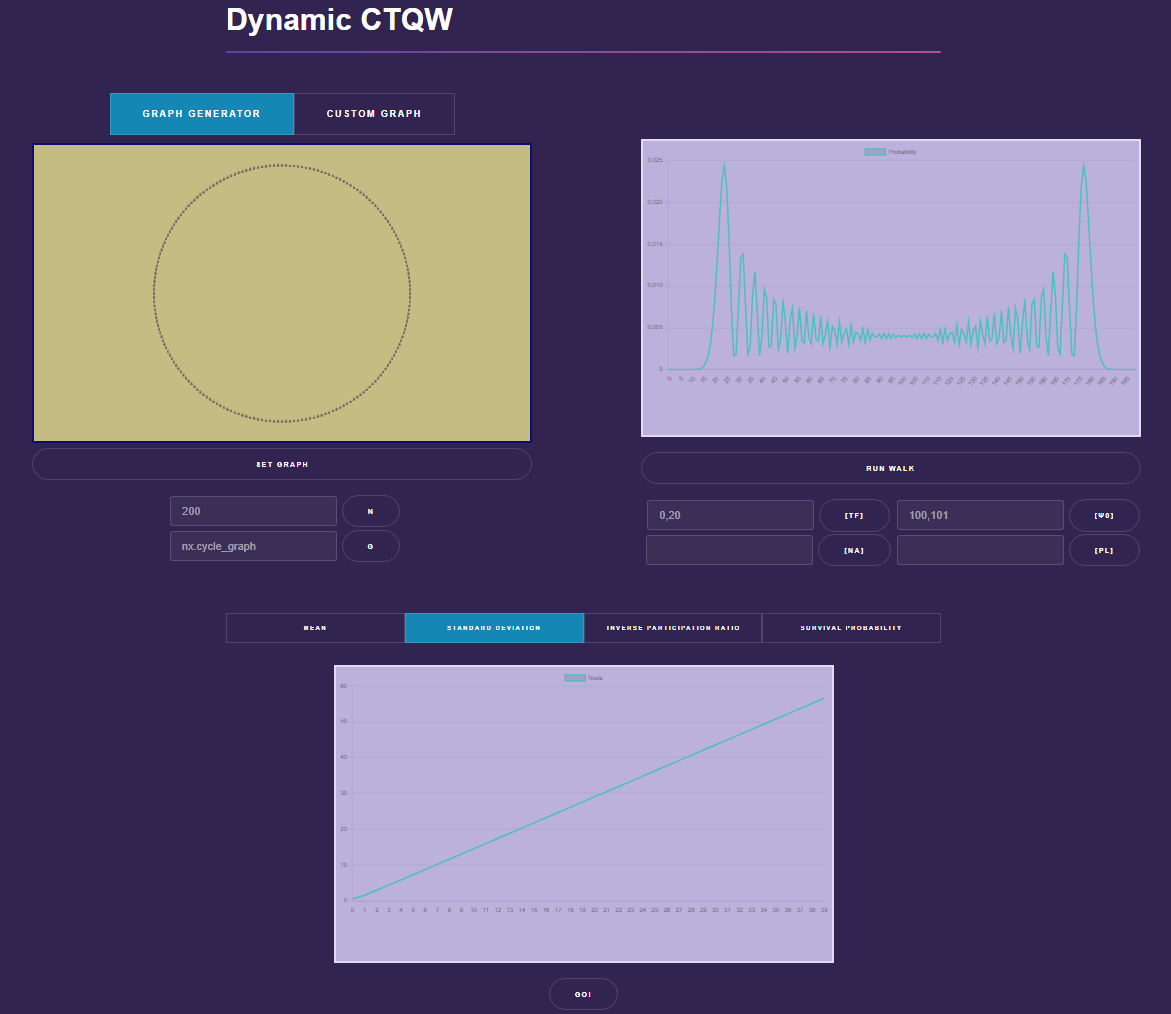
\includegraphics[scale=0.4]{img/QWAK/qwakGuiDynamicQW.png}
  \caption{Graphical interface page of the dynamic continuous-time quantum walk evolution.}
  \label{fig:guiDynamicPage}
\end{figure}

For dynamic visualization of the walk, figure \ref{fig:guiDynamicPage} displays
the corresponding page. Graph creation is identical to the static case, however
the probability distributions will not be a simple plot but an animation.
Instead of inputting a single time value, the user should enter a lower and
upper limit for the time interval. By pressing the \textit{Run Walk} button,
the user now calls \texttt{buildWalk} as many times as the interval specifies,
after which \texttt{ChartJS} will plot multiple arrays of probability
distributions contained in a list, effectively animating the evolution of the
quantum walk. Because every probability distribution has a particular value for
each transport property, we provide a plot of the evolution of these
values instead. Figure \ref{fig:guiDynamicPage} then shows the typical ballistic
behavior of the quantum walk since its standard deviation evolves linearly in
time. 

This concludes the description of the \texttt{QWAK} package. In the future, we
would like to expand our Python package with the ability to perform the CTQW
with multiple walkers since they may show interesting and unexplored transport
properties. Visualization tools for the backend will also be explored, such as
adding methods for creating plots of interesting relationships between the
various parameters of the walk, and also an easy way of creating animations
without using the GUI. Another major feature will be to include the stochastic
quantum walk in the graphical user interface, which was not done in this
version due to it being a recent addition to the package. Other minor changes
to the software will include improvements to the performance of the \texttt{checkPST}
method, and the \texttt{StochasticQWAK} class, since they are the most resource
intensive routines. 


\end{document}
